\documentclass[tikz,border=6pt]{standalone}
\usepackage[T1]{fontenc}
\usepackage[utf8]{inputenc}
\usepackage{pgfplots}
\usepgfplotslibrary{groupplots}
\usetikzlibrary{calc}
\pgfplotsset{compat=1.18}
\begin{document}
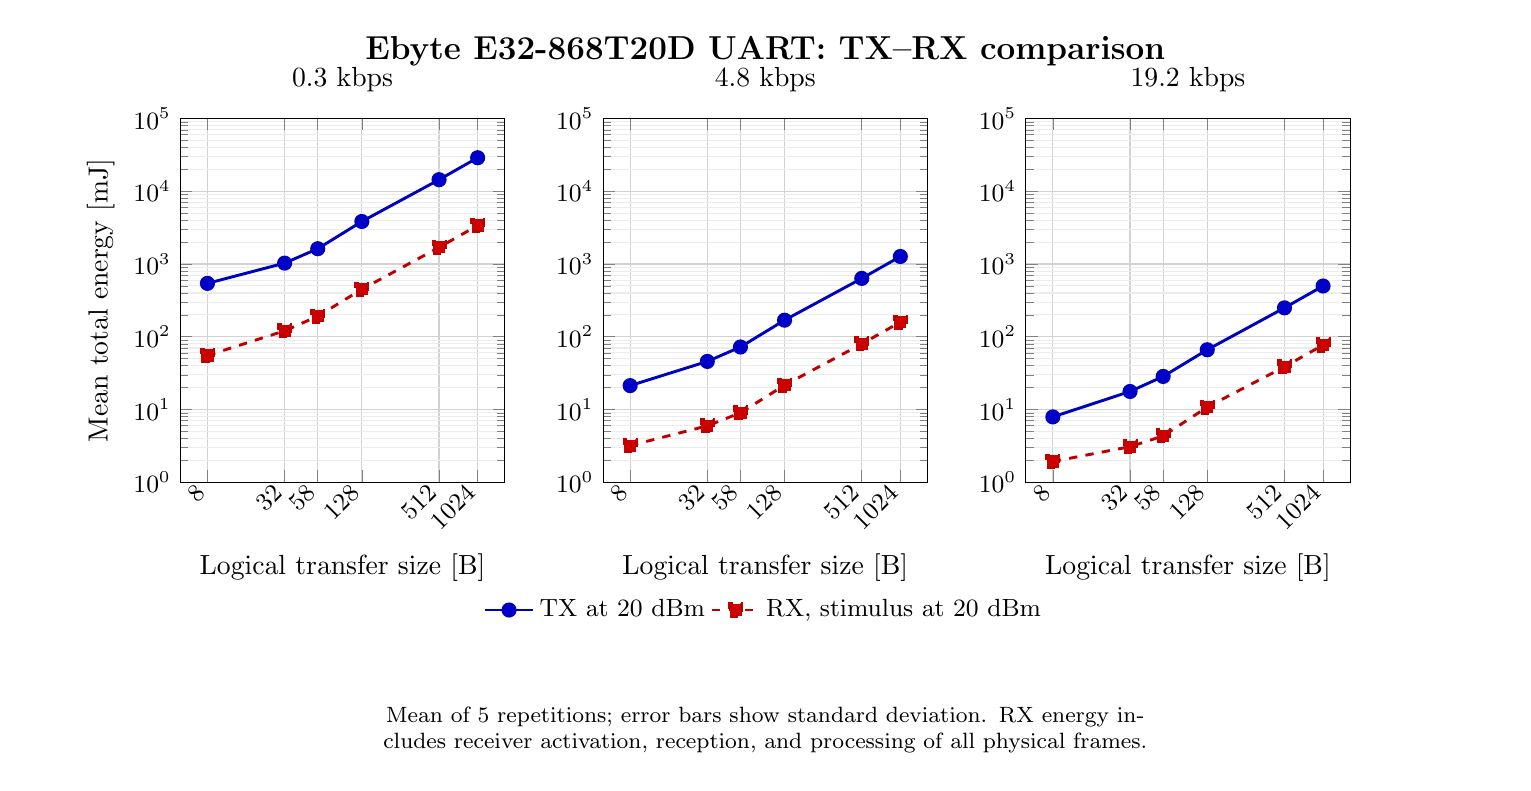
\begin{tikzpicture}
\begin{groupplot}[/pgf/number format/use comma,
  group style={group size=3 by 1, horizontal sep=1.25cm},
  width=5.7cm, height=6.2cm,
  xmode=log, log basis x={2}, ymode=log, log basis y={10},
  ymin=1, ymax=100000,
  xtick={8,32,58,128,512,1024}, xticklabels={8,32,58,128,512,1024},
  x tick label style={rotate=45, anchor=east, font=\small},
  y tick label style={font=\small},
  grid=both, minor grid style={gray!15}, major grid style={gray!35},
  xlabel={Logical transfer size [B]},
  every axis plot/.append style={line width=1.05pt},
  error bars/error bar style={line width=0.35pt},
  legend style={font=\small, draw=none, fill=none, at={(0.5,-0.29)},
    anchor=north, legend columns=-1},
]
\nextgroupplot[title={0.3 kbps}, ylabel={Mean total energy [mJ]}]
\addplot+[color=blue!75!black, solid, mark=*, mark size=2.2pt,
  error bars/.cd, y dir=both, y explicit,
] coordinates {
  (8,542.077683) +- (0,0.476680879)
  (32,1029.33218) +- (0,1.4044938)
  (58,1624.89807) +- (0,2.05573686)
  (128,3846.02637) +- (0,2.94000291)
  (512,14447.2025) +- (0,13.1733198)
  (1024,28958.0312) +- (0,32.4301291)
};
\addplot+[color=red!75!black, dashed, mark=square*, mark size=2.2pt,
  error bars/.cd, y dir=both, y explicit,
] coordinates {
  (8,55.2473702) +- (0,0.0735274203)
  (32,120.607927) +- (0,0.0604488262)
  (58,191.558293) +- (0,0.0799205841)
  (128,449.067292) +- (0,0.250957906)
  (512,1695.0262) +- (0,0.492855456)
  (1024,3389.34179) +- (0,0.382176861)
};
\nextgroupplot[title={4.8 kbps}]
\addplot+[color=blue!75!black, solid, mark=*, mark size=2.2pt,
  error bars/.cd, y dir=both, y explicit,
] coordinates {
  (8,21.2945275) +- (0,0.0302056589)
  (32,45.8073506) +- (0,0.170395694)
  (58,72.3133997) +- (0,0.237277791)
  (128,169.02978) +- (0,0.553425085)
  (512,634.409172) +- (0,0.949392434)
  (1024,1269.81883) +- (0,0.974012847)
};
\addlegendentry{TX at 20 dBm}
\addplot+[color=red!75!black, dashed, mark=square*, mark size=2.2pt,
  error bars/.cd, y dir=both, y explicit,
] coordinates {
  (8,3.18526471) +- (0,0.00357652102)
  (32,5.96819925) +- (0,0.00822816774)
  (58,8.98010075) +- (0,0.0153784074)
  (128,21.6161486) +- (0,0.0363333427)
  (512,79.6617814) +- (0,0.0559019751)
  (1024,159.241008) +- (0,0.0669143106)
};
\addlegendentry{RX, stimulus at 20 dBm}
\nextgroupplot[title={19.2 kbps}]
\addplot+[color=blue!75!black, solid, mark=*, mark size=2.2pt,
  error bars/.cd, y dir=both, y explicit,
] coordinates {
  (8,7.91120402) +- (0,0.0101505503)
  (32,17.6863226) +- (0,0.0301411057)
  (58,28.4690745) +- (0,0.0800841039)
  (128,66.3184263) +- (0,0.211907672)
  (512,249.792515) +- (0,0.517092667)
  (1024,498.822931) +- (0,1.06865604)
};
\addplot+[color=red!75!black, dashed, mark=square*, mark size=2.2pt,
  error bars/.cd, y dir=both, y explicit,
] coordinates {
  (8,1.92568591) +- (0,0.00103364787)
  (32,3.0805547) +- (0,0.0037965628)
  (58,4.32723918) +- (0,0.00565236146)
  (128,10.8049593) +- (0,0.00922745563)
  (512,38.6512439) +- (0,0.0316200881)
  (1024,77.0587849) +- (0,0.0910455986)
};
\end{groupplot}
\node[font=\bfseries\large] at ($(group c2r1.north)+(0,0.85cm)$)
  {Ebyte E32-868T20D UART: TX--RX comparison};
\node[font=\footnotesize, align=center, text width=18.5cm]
  at ($(group c2r1.south)+(0,-3.15cm)$)
  {Mean of 5 repetitions; error bars show standard deviation. RX energy includes receiver activation, reception, and processing of all physical frames.};
\end{tikzpicture}
\end{document}
